\chapter[A GUI for the Experiment]{Building a Graphical User Interface for the Experiment}\label{building-a-graphical-user-interface-for-theexperiment}

\section{Objectives}
Building {GUI}'s is a very rewarding experience because you will really
see the outcome of your program. It is much more impressive to show to
someone a beautiful window with a couple of buttons than hundreds of
lines of code. When you develop a working User Interface, you will
really have the feeling of delivering an end-product. A window pops up,
an error message appears, an experiment is performed. In this chapter,
you will learn the steps needed for designing a window and plotting the
data acquired by a device. The chapter involves some design, some coding
and a lot of thinking. It is strongly advised to drive inspiration from
the examples in case you get stuck for too long in one of the exercises.

\section{Introduction}
Building GUIs may seem more complicated than what it really is. It is,
of course, not an easy task but once you get the fundamentals you will
see that, as with any other skill, it is possible to learn. Most
experiments can be performed right from the command line, as you have
seen in the previous examples. You can have a great level of control
running a Python script, or import your models into a Jupyter notebook.
However, in some cases, it can be very handy to control the parameters
of an experiment and to monitor the output in a window
especially designed.

There are several options for building GUIs with Python. For example, in
the previous chapter, you have already seen how to plot the data while
the experiment is running. It is a bit rudimentary but it is indeed a
\emph{user interface}. In this chapter, we are going to focus on one
particular library for building interfaces called \textbf{Qt}. Qt was
developed as an application framework that allows developers to build
apps that look native in different systems without changes to the code.
This means that if you develop an application and run it on Windows it
will look like a Windows program, but the exact same application will
look like a Linux program if you run it on such a computer.

Moreover, Qt comes with a lot of interesting features to connect
different parts of your code. For example, when moving a slider in the
{UI}, the value of a parameter in your experiment model should change.
Qt also provides the tools you need to create all the elements that a
program needs, from menus to buttons and the flexibility to define your
own elements, such as a plot. Qt was not developed with Python in mind,
but fortunately, some projects have advanced a lot in making it
compatible. There are mainly two, called
\href{https://riverbankcomputing.com/software/pyqt/intro}{PyQt} and
\href{https://wiki.qt.io/PySide}{PySide}. The difference between them is
the license under which they are released. If licenses are a concern for
you, for example, because you are developing commercial software, you
should definitely check their differences. In the case of this book, we
are going to use PyQt5 because the programs we are developing have no
commercial interests.

You have to be aware that the current version of Qt is \textbf{Qt5}, and
therefore the examples in this and the next chapter are based on
\textbf{PyQt5}. However, up to some years ago, the most spread version
was \textbf{Qt4}. There is no backward compatibility between them,
meaning that code that worked with \textbf{PyQt4} not necessarily will
work with \textbf{PyQt5}. It is very important that you don't mix both
libraries. If there are applications on the computer where you are
developing the code that depends on \emph{PyQt4}, it is very important
to isolate your development with a Virtual Environment, as explained in
Chapter 02.

In this chapter, you will find some design and some coding. Up to now,
it was simple to include the code in the book for you to see, however,
design files are not \emph{copy/pasteable}. All the design files are
available for you to download from the Github Repository.

\hypertarget{simple-window-and-buttons}{}
\section{Simple window and buttons}\label{simple-window-andbuttons}

Now it is finally time to start using the empty folder from the M
\textbf{V} C design pattern: the \textbf{View}. The folder will be a
python module, and thus it needs a \mintinline{python}{__init__.py} file, like
all other modules. Inside the \textbf{View}, create a folder called
\mintinline{python}{GUI} where you are going to store the files that build the
windows. Soon enough, you will see that when you work with Qt you will
have two different types of files. One will be the way the program looks
and will have \emph{.ui} as the extension. Then, you will have the
Python modules responsible for building up the interface.

You will start by designing a simple window with two buttons, one to
start and the other to stop a scan. You will also add a line where you
can see if the scan is running or not. The first step is to open the
program \textbf{Qt Designer}, which was installed in Chapter 02. The
program will welcome you with a window like the one below:

\begin{center}
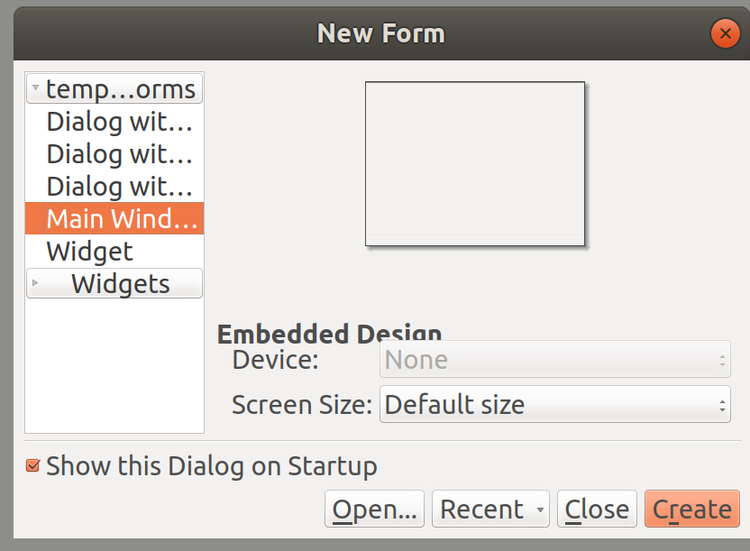
\includegraphics[width=.6\textwidth]{images/qt_designer_welcome.png}
\end{center}

Since you are creating your first window, you have to select \emph{Main
Window} as displayed. Don't worry too much about the technicalities at
this stage, it is important that you start going and you will slowly get
the concepts later on. The only important thing to know now is that in
Qt, \emph{widgets} are the building blocks of any user interface. A
button is going to be a widget, a plot, slider, etc. are all widgets Now
you can start playing around with the designer, and familiarize yourself
with it.

\exercise{Generate a window that looks like the image.
\begin{center}
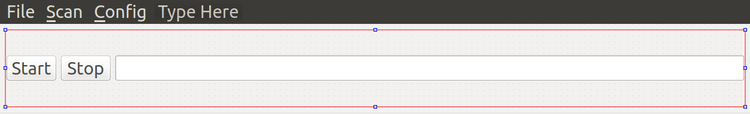
\includegraphics[width=.6\textwidth]{images/main_window.png}
\end{center}}


If you look closely, you will notice a menu as well, at the top, called
\emph{File}. For the time being it is optional, but you will need the
menu later on. The designer has a lot of options that can be useful, for
example specifying the layout. The layout is a way in which objects are
going to be arranged in the window; a vertical layout means that
different objects are going to be stacked one under the other. You can
also find a horizontal layout, a grid layout, and a form layout. Feel
free to explore how they behave. Remember that you can nest them for
enhanced flexibility. It is also possible to work without layouts,
specifying the exact position and size of each widget in the window. As
you can see, Qt doesn't impose design restrictions, it is really up to
you to decide what and how to build things.

\exercise{Nest a horizontal layout (for the buttons) within a vertical layout that
later on will hold the plot of the data.
\begin{center}
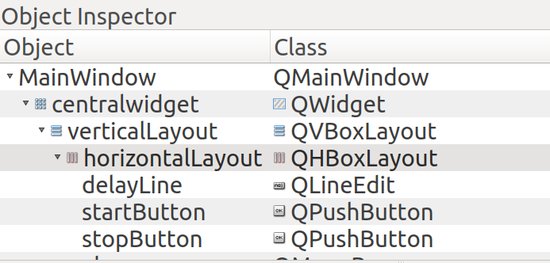
\includegraphics[width=.6\textwidth]{images/nested_layouts.png}
\end{center}}

\exercise{Improve the window to look like the image. This is going to be the entry
point for your program, and from here you are going to configure and
trigger scans.

\begin{center}
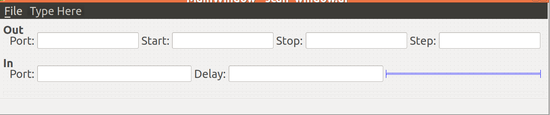
\includegraphics[width=.6\textwidth]{images/scan_window.png}
\end{center}}

At this point, you have an idea of what can be done with Qt Designer,
but what you need to learn now is how to give different functionalities
to the different widgets on the screen. There is, however, something
important to pay attention when dealing with the designer. The names
that you assign to each widget is going to be the way to identify it
also within Python. However, it is very complicated to find out the name
you gave to each element from the designer file, it is much easier and
faster doing it directly from within the program itself. Since now you
will be dealing with files coming from two different sources, i.e.,
Python files generated in an editor and designer files, it is very
important that the naming conventions are consistent. If you are in
doubt, or you see some bugs that you find to resolve, you can always
download the files from the
\href{https://github.com/PFTL/SimpleDaq/tree/master/PythonForTheLab/View/GUI}{Github
repository}.

\note{If you look for documentation online on how to use PyQt in your
applications, you most likely will find that you should compile the
\mintinline{python}{uic} designer files into a python file, that you can import as
any other module. This step is not at all necessary and will just add
more difficulty to an already complicated process. Rendering the uic
file directly in your code is much simpler, faster and more robust in
the long term.}

The best idea is to start simple. You are going to write a script that
can generate and open an empty window. First, create a file called
\textbf{simple\_open\_window.py} within the \textbf{Examples} folder and
add the following to it:

\begin{minted}{python}
import sys

from PyQt5.QtWidgets import QApplication, QMainWindow

app = QApplication(sys.argv)
m = QMainWindow()
m.show()
app.exit(app.exec_())
\end{minted}

If you run this script, you will see a window popping up in all its
splendor. Let's see what is actually happening line by line. The
\mintinline{python}{sys} module is responsible for everything that involves the
operating system, as you shall see later. Then you import two modules
from the PyQt5 library. You have to understand that in PyQt everything
always starts with a \mintinline{python}{QApplication}. You have to start an
application before you can open a window or create widgets. You also
import \mintinline{python}{QMainWindow} which is the widget that is going to hold
all the design elements needed for an application.

Every PyQt program will start in the same way. First, you define the
\mintinline{python}{app} using the module \mintinline{python}{QApplication}. Pay attention to
the fact that it takes one argument, in this case, \mintinline{python}{sys.argv},
which is a list of the commands passed when executing the script from
the command line. For example, if you run the script as
\mintinline{bash}{python script.py -option test}, you will have a list in
\mintinline{python}{sys.argv} stating that the \emph{option} you used is
\emph{test}. PyQt allows you to specify some parameters, such as the
style of the app. However, even if you are not going to use them, you
have to specify an argument, and better be consistent throughout
different programs.

In the next couple of lines, you create a \mintinline{python}{QMainWindow}, which is
also what you have done in the Designer. You can already start seeing
that there are two ways to achieve the same results, one is
programmatically, writing the code to generate Qt windows and the other
is graphical, with programs such as Qt Designer. After you've created
the \emph{Main Window}, you need to make it appear with the
\mintinline{python}{show()} command. If you have ever used \emph{Matplotlib} you can
see the similarities.

Finally, you have run the \mintinline{python}{app}. Check that you do it in a nested
way, you call \mintinline{python}{app.exit} and as an argument, you use
\mintinline{python}{app.exec_()}. An App in PyQt can be thought of as an infinite
loop that will keep every piece of the Qt program running. Normal Python
scripts exit when they are done, but a {GUI} needs to run until you stop
it. This is what \mintinline{python}{app.exec_()} does. By passing it as an
argument to \mintinline{python}{app.exit} you can be sure that for whatever reason
the execution is interrupted, the application process will be stopped.
It is a safe way of terminating an application, which can be very
important if you are running large projects.

Of course, a simple, empty window, is not what you are after. What is
important to note is that if you run the same script on different
computers, the outcome will be slightly different. The look and feel of
every window will match with your operating system, this is one of the
many advantages of using Qt. A good way of expanding the code is by
including the file that you have developed with the designer.

\begin{minted}{python}
import sys
import os

from PyQt5.QtWidgets import QApplication, QMainWindow
from PyQt5 import uic

app = QApplication(sys.argv)
m = QMainWindow()
file_dir = '/home/user/programs/PythonForTheLab/PythonForTheLab/View'
uic.loadUi(os.path.join(file_dir, 'GUI/scan_window.ui'), m)
m.show()
app.exit(app.exec_())
\end{minted}

The core of the script is the same as before, the new lines are for
establishing the path of the \emph{View} folder and to load the design
file. You will see a better way of doing this in the program, but for
the time being it works well. Go ahead and run the script. You will see
that the window is displaying the design that you had generated. You
should be proud of yourself. There is a good chance that this is the
first time that you actually have an application written from scratch by
yourself and running on your own computer.

\section{Adding buttons and interaction}\label{adding-buttons-andinteraction}
Now you have a window that may look great but it is not doing anything.
You need to start building your code in order to allow actions to be
triggered by pressing a button, for example. But for having code that
is reusable and expandable, you have to rewrite your previous example.
You will need to define a new class that inherits from
\mintinline{python}{QMainWindow} and that allows you to personalize it as much as
you want. You have to create a new file within the \textbf{View} folder
and call it \textbf{scan\_window.py}. You can adapt the previous example
like this:

\begin{minted}{python}
from PyQt5 import QtWidgets, uic

class MainWindow(QtWidgets.QMainWindow):
    def __init__(self, parent=None):
        super().__init__(parent)

        p = os.path.dirname(__file__)
        uic.loadUi(os.path.join(p, 'GUI/scan_window.ui'), self)

if __name__ == '__main__':
    app = QApplication(sys.argv)
    m = MainWindow()
    m.show()
    app.exit(app.exec_())
\end{minted}

As you can see, the code after \mintinline{python}{if __name__} is almost the
same than what you have done before. If you execute the file, you will
notice that the window is opened with the design. Going back to the new
class you have defined, you can see that it inherits from the
\mintinline{python}{QMainWindow} class, because what you are developing is the main
window of your program. The \mintinline{python}{__init__} method should always
take one argument called \mintinline{python}{parent} because it is used by Qt to
keep track of the relationship between widgets. When you use the
\mintinline{python}{super()} to initialize the parent class, you need to pass the
same parent.

You can see that the way to import the designer file is slightly
modified. Since you need to perform a relative import, the first step is
to establish the location of the current file, and that is what you do
when you call the \mintinline{python}{__file__} property. Next, you append the
path to the \emph{ui} file to the location of the
\textbf{scan\_window.py} file and load it, as what you have done before.
When you want to import files within Python, you have to specify
precisely where they are located. Working with relative imports is not
always safe with Python, especially for larger projects. Sometimes to
root folder is not the folder that contains the file, but the folder
from which you trigger the program. That is why it is always safer to
use absolute paths for imports and not just relative ones.

Once you have a subclass of \mintinline{python}{QMainWindow}, you will have complete
control over what happens in the window, where the user is clicking, you
will also be able to add new elements, to update them, etc. The advantage of defining a new class is that you can reuse it in different
projects and that it can be easily embedded into larger programs. For
the time being, you only want to do a scan, but it can be that tomorrow
the scan is only a part in a larger series of experiments and the main
window becomes just one more window.

One of the building blocks of any app is buttons. However, if you
downloaded the example design file from the Github repository, you will
notice that there are no buttons in it, just a container called
\mintinline{python}{buttonBox}. First, you will learn how to add elements to the
{GUI} directly from the Python code, then you are going to learn how to
trigger actions when a button is pressed. The logic behind Qt elements
is that first, you initialize them, then you add them to the position
where you desire and then you program how they are going to behave.
Let's first create two buttons, one start, and one stop. You should add
the following the to \mintinline{python}{MainWindow} class:

\begin{minted}{python}
self.startButton = QtWidgets.QPushButton('&Start')
self.stopButton = QtWidgets.QPushButton('S&top')
self.buttonBox.addButton(self.startButton, 
            QtWidgets.QDialogButtonBox.ActionRole)
self.buttonBox.addButton(self.stopButton, 
            QtWidgets.QDialogButtonBox.ActionRole)
\end{minted}

The string specified when declaring the buttons is the text that will
appear in them. Adding an \mintinline{python}{\&} before a letter is just for
enabling the user to quickly reach the button by pressing Alt+S or Alt+T.
The next couple of lines are for adding the buttons to the
\mintinline{python}{buttonBox}. You can add the buttons to any layout that you have
specified within the designer. The main difference is that the method
you have to use is \mintinline{python}{addWidget} and takes only one argument, the
widget (in this case the button) that you wish to add.

\exercise{Create a designer file with different layouts and add buttons to each,
in order to see how they behave.}

Now that the buttons are ready in the {GUI}, let's start with a very
simple idea: printing to the terminal \mintinline{text}{'Button Pressed'} when a button
is pressed. To achieve this, you have to understand one of the most
powerful components of Qt programming: \textbf{Signals}. A signal is
what enables you to capture an event and trigger an action. You can hook
those signals to one or more functions (also called \emph{Slots}) and Qt
will take care of executing them when appropriate. If you remember, the
\mintinline{python}{QApplication} can be regarded as an infinite loop, taking care
of the behavior of the applications, including the connection between
\emph{Signals} and \emph{Slots}.

In Qt, there are a lot of different signals that get fired at very
precise moments. For example, when you click with the mouse on a button
it will generate a specific signal. But it is not the only one. Moving
the mouse, releasing a button, hovering over an element, the list goes
on and on. You can even trigger your own signals with your own
conditions, for example when the user presses a specific combination of
keys while moving the mouse. But before getting too complicated, let's
just start adding some action when clicking the \mintinline{python}{startButton}.
Update the Main Window class with the following line of code and
function:

\begin{minted}{python}
class MainWindow(QtGui.QMainWindow):
    def __init__(self, parent=None):
        [...]

        self.startButton.clicked.connect(self.button_clicked)

    def button_clicked(self):
        print('Clicked')

    [...]
\end{minted}

If you just run the file and click on the start button, you will see
that there is a message being printed to the terminal. What is happening
is that the \mintinline{python}{startButton} has a \mintinline{python}{signal} called
\mintinline{python}{clicked} and you have connected that signal to the method
\mintinline{python}{button_clicked}. Bear in mind that you don't put the
\mintinline{python}{()} when you connect the signal, you are interested in just the
method. \mintinline{python}{button_clicked} is very simple, it only prints to
screen a message when it is executed. This example looks a bit basic,
but if you have been following all the way, you can realize that
triggering a scan is just calling the proper \mintinline{python}{Experiment} method.

\exercise{There are other signals for a \mintinline{python}{QPushButton}, for example
\mintinline{python}{released} and \mintinline{python}{pressed}. Hook them up to your own methods
and play around. When is the \mintinline{python}{released} signal triggered? And the
\mintinline{python}{pressed}?}

If you want to know which signals are available and which method does
every QtWidget possess, you can refer to the
\href{http://doc.qt.io/qt-5/qtwidgets-module.html}{Qt documentation}. It
is the official documentation and therefore the syntax is for C++, but
you can easily adapt it to Python, especially if you follow the examples
outlined in this book.

\section{Hooking the Experiment to the GUI}\label{hooking-the-experiment-to-the-gui}
It is time to start interacting with your device straight from the
{GUI}. Create a new file called \textbf{start\_gui.py} in the
\textbf{Examples} folder just next to \textbf{start\_cli.py}. You will
put together everything what you already know. The idea behind having a
class for the experiment is that you can instantiate and pass it to the
{GUI} as arguments to the different windows. For example, this is how
the \textbf{start\_gui.py} will look like:

\begin{minted}{python}
import sys
from PyQt5.QtWidgets import QApplication

from PythonForTheLab.Model import Experiment
from PythonForTheLab.View.scan_window import ScanWindow

e = Experiment()
e.load_config('Config/experiment.yml')
e.load_daq()

ap = QApplication(sys.argv)
m = ScanWindow(e)
m.show()
ap.exit(ap.exec_())
\end{minted}

This example is exactly a merge of both previous examples, the
\emph{CLI}, and the \emph{GUI}. Pay special attention to the
highlighted line. You are passing the experiment class to the
\mintinline{python}{ScanWindow}, but \mintinline{python}{ScanWinow} class does not take
arguments other than its parent. If you run that file now it will give
an error, however, feel free to go ahead and try, you will see that the
error is very descriptive. Note also that you are passing the Experiment
already instantiated, with the configuration and the daq loaded. It is a
matter of convenience, and not of necessity. You will see later that
those two actions can also be triggered from within the {GUI}.

In order to accept the experiment as an argument, you need to update the
code of the \mintinline{python}{ScanWindow} class.

\begin{minted}{python}
class ScanWindow(QtGui.QMainWindow):
    def __init__(self, experiment=None, parent=None):
        super().__init__(parent)
        self.experiment = experiment
    
    [...]
\end{minted}

Note that you have specified a default value for the experiment
variable: \mintinline{python}{None}. This trick is very important when you are
refactoring a class or a function. Imagine you have a large project and
you are using the \mintinline{python}{ScanWindow} in different locations, or even
more importantly, your package is used by someone else. If you just add
the experiment as an argument, what will happen is that any piece of
code that looks like \mintinline{python}{ScanWindow()} will throw an error. This
implies changing the code in every line that has used the class. If you
add a default value, you guarantee that older code is still compatible.
For larger changes, however, this may not be sustainable.

\warning{It is not possible to maintain backward compatibility always. In the
example that you are developing, the experiment is going to become a
very important piece. Older code that doesn't supply an experiment
object will eventually lead to something broken downstream.}

\exercise{Now the experiment class is stored as \mintinline{python}{self.experiment}; can you
replace the method \mintinline{python}{clicked} in order to print the \mintinline{python}{idn}
of the daq card?}

\exercise{Replace the behavior of the start button. Trigger a scan with the
parameters already stored in the experiment. What happens to the {GUI}
if you do so? \textbf{warning}: I suggest you use parameters in the
{YAML} file that make your total scanning time relatively short.}

\section{Threads to the Rescue}\label{threads-to-therescue}
If you have finished the last exercise, you probably noticed that while
the scan is running your {GUI} freezes. Depending on your operating
system and the time it takes the scan to run, you will get a
notification saying that your app does not answer and you will be asked
if you would like to terminate it. It means that you need to find a way
to prevent long-running tasks from interrupting the main loop of our
Application. After all, you don't see Firefox freezing every time a page
takes a bit longer to load, or your photo editing software when it
exports the pictures with a new resolution.

The way in which Python programs can handle this is with the use of
threads. When you run a script, everything is going to happen from top
to bottom, one line at a time. If a function takes too long to execute
it will be halted there. Remember that taking too long doesn't mean it
is computer intensive work. For example, you can be waiting for user
input, or perhaps you want to trigger something every 10 minutes and you
put a \mintinline{python}{sleep} statement. Threads are a way of handling this
behavior, by allowing several processes to run simultaneously. In our
case, we want our scan experiment to run in a thread separated from the
thread in which the main {GUI} is running.

\note{If you finished the last chapter, you have already learned how to work
with threads in Python. Working with threads in Qt follows basically the
same principles, but with the added benefits of signals and slots. It
is, normally, a good idea not to mix Python threads and Qt threads
when possible.}

Working with threads in Qt is relatively easy, especially thanks to
\emph{Signals}. First, you need to create is a new class that you are
going to call \mintinline{python}{WorkerThread}. Workers are going to run whatever
method you give them to run but will do so in a separate thread. You
should create a new file in the \textbf{View} folder and call it
\textbf{general\_worker.py}. The idea of calling it \emph{general} is
because it will run any function you want. Worker threads can also be
specialized, meaning that they will take care, for example, of the
acquisition of a camera, the input from a user, etc.

\begin{minted}{python}
from PyQt5 import QtCore

class WorkThread(QtCore.QThread):
    def __init__(self,  function, *args, **kwargs):
        super().__init__()
        self.function = function
        self.args = args
        self.kwargs = kwargs

    def __del__(self):
        self.wait()

    def run(self):
        self.function(*self.args,**self.kwargs)
        return
\end{minted}

When working with Qt threads, you need to reimplement some important
methods and that is why this class may look particularly complicated.
You start by creating a new class called \mintinline{python}{WorkerThread} that
inherits the QThread class. The \mintinline{python}{__init__} method takes one
required argument, called \mintinline{python}{function}, which is the function that
the thread is going to execute. \mintinline{python}{*args} and \mintinline{python}{**kwargs} is
just a way of accepting any number of variables. You don't know exactly
how many arguments the function is going to take since it can
\emph{a-priori} be any function. You store all the information as
properties of the class (\mintinline{python}{self.function}, etc.). The
\mintinline{python}{__del__} method is there just to be sure that the Thread is
properly closed if you decide to stop it before it finishes running.

The important part of the code is the \mintinline{python}{run} method. This method
is going to be called from the main part of the code when we want to
execute it. In this specific case, you just execute the function that
you passed at the beginning while instantiating the class. Notice that
you are passing to the function the same arguments that the
\mintinline{python}{__init__} took, namely \mintinline{python}{*args} and \mintinline{python}{**kwargs}.
Once the class is ready, it is time to see how to use it from the main
code. If you go back to the \textbf{scan\_window.py}, you will need to
update the code to run the thread properly. If you finished last
section's exercise, you should have ended up with code like this:

\begin{minted}{python}
def button_clicked(self):
    self.experiment.do_scan()
\end{minted}

Since you are trying to do proper coding, you need to update the names
of the methods for them to make sense. For example, you can have a new
method called \mintinline{python}{start_scan} that will look like this:

\begin{minted}{python}
def start_scan(self):
    self.worker_thread = WorkThread(self.experiment.do_scan)
    self.worker_thread.finished.connect(self.worker_thread.deleteLater)
    self.worker_thread.start()
\end{minted}

Remember to update the code where you are connecting the signal
\mintinline{python}{clicked} of the start button to the method. First, note that you
created a \mintinline{python}{worker_thread} as a property of the
\mintinline{python}{ScanWindow} but was not defined within the \mintinline{python}{__init__}
method, which is violating some design principles but you can still deal
with it. The only argument that you are passing to the thread is the
function that you want to execute, in this case, \mintinline{python}{do_scan}. Pay
attention to the fact that you are passing the function without
\mintinline{python}{()}. If you add the \mintinline{python}{()} you would pass the result of the
function and thus you will have to wait until it finishes for creating
the \mintinline{python}{worker\_thread}. Then you connect the signal
\mintinline{python}{finished} from \mintinline{python}{worker_thread} to one of its own
methods. It can be slightly convoluted, but this will ensure that when
the thread finishes it is going to be cleared. If you run the same
program for months you really don't want to start accumulating in memory
millions of garbage threads. Finally, you \mintinline{python}{start} the thread. Pay
special attention to the fact that you don't use the \mintinline{python}{run} method
explicitly. You can go ahead and run the program again. Is it still
freezing when you perform a scan?

\exercise{You have only the start button working. Hook the stop button to a new
method \mintinline{python}{stop_scan}. To stop the execution of a thread you have
to use the \mintinline{python}{quit()} method, for example:
\mintinline{python}{self.worker_thread.quit()}.}

\exercise{Thanks to what you have developed in the previous chapter, you can also
stop the scan by changing the value of a property. Update the
\mintinline{python}{ScanWindow} to use it.}

\exercise{How can you prevent the program from trying to stop a thread that is not
actually running? A great idea would be to add a property called
\mintinline{python}{self.scan\_running} and set it to \mintinline{python}{False} in the
\mintinline{python}{__init__}, set to \mintinline{python}{True} when you start the scan and
back to \mintinline{python}{False} when the scan ends. Try to implement this in your
code.}

\exercise{Prevent the user from triggering two scans at the same time, for
example, you can disable the start button by using the method
\mintinline{python}{setEnabled(False)} or \mintinline{python}{setEnabled(True)}}

\section{Conclusions}\label{conclusions}
This chapter may have been one of the more interesting and compelling
chapters in the book. You have built a user interface and you have
hooked an experiment to it. The {GUI} is far from complete, but
nevertheless, it is a great achievement what you have developed so far.
With what you have done here you can already do plenty of things if you
are creative enough. You can have a user interface for triggering
actions on your computer, in your experiment, etc. The options are
endless and you are only halfway through, so imagine what is going to
happen next.

\subsection{A Word on Qt}\label{a-word-onqt}
Qt was developed for C++ programmers and was later ported to Python.
This means that a lot of the documentation and examples that you can
find around are for another language and thus you will need to translate
it into Python. If there is something you can't understand and there are
no obvious answers online, ask in
\href{https://forum.pythonforthelab.com}{Python For The Lab}, the community over there is very helpful and knowledgeable.

When developing programs, normally you read code from top to bottom, one
line at a time. This is also what computers do when interpreting or
compiling programs. When you start dealing with \emph{user interfaces}
it becomes almost impossible to read code from top to bottom. For
example, you never know when a user will trigger an action, stop it, in
which order, etc. That is why the last exercise of the previous example
is very important. You should anticipate, at least to a certain extent,
the mistakes that a user can commit.

Of course, there are also limits to how much you can anticipate. When
developing programs for the lab, normally you assume that the users of
your code are going to be aware of what they are doing and how the
experiment is designed. However, more often than what you think,
mistakes happen. Perhaps even yourself forget about a detail, or you are
in a hurry to acquire the last few data points. Therefore, thinking
ahead about common mistakes and displaying appropriate messages can save
you and the users of your program a lot of time later on.

Getting to understand how Qt works and how you can do different things
with it is a lengthy process. Every app that you see, not only on your
computer but also on your mobile phone or embedded platform such as
smart watches or thermostats can be built using Qt. It is completely up
to you to put a limit on what you need to learn in order to perform an
experiment. Do you want to make the interface prettier with icons? Do
you want to verify the user input and display warning messages? Do you
want to stream a camera signal? All those are possibilities few keyboard
strokes away, but they are of course much more involved than what you
have developed until now.

\subsection{A Word on Signals}\label{a-word-onsignals}
Working with \emph{Signals} is incredibly handy, and once you get used
to them you will want them to be available everywhere, especially when
you are doing some threading in Python. However, signals make your code
harder to follow for beginners. You connect your signal once and you
forget about it. Every time a signal is fired, something will be
triggered, such as a method or a function. Checking what is called and
which arguments are being passed becomes more complicated. Even the best
IDEs available for Python won't be able to track what is really
happening in your code.

If you are developing code that you expect others to understand, you
should either provide all the documentation they need or limit the number of nonordinary packages that you are employing. For example, if
the users of your code are used to analyzing data, you can count on them
knowing \emph{numpy} and \emph{matplotlib}, but most certainly they are
not aware of \emph{PyQt} and its special models such as \emph{signals}
and \emph{slots}. If you are building code for others, be sure you use
libraries common to them when possible, or document your progress to
make it understandable.
